The definition of D-reducibility required that every ring coloring was reconfigurable to a valid coloring of $\overline{\Phi}(\confg)$. If this is not possible, we must avoid the unfixable colorings. In Section \ref{sec:reducers} we introduced reducers to guarantee certain ring colorings for use in proofs. These reducers constrain which ring colorings can be encountered on the ring of the original configuration. Therefore, we may apply them in the same manner for individual configurations to avoid unfixable colorings in D-reducibility. This results in what is known as C-reducibility.

\subsection{Definition with Bernhart's Diamond}

We will be working with an example as we develop this theory. This example is a relative of the Birkhoff Diamond ($
\bir$), called the Bernhart Diamond ($\ber$). First proven to be reducible by Arthur Frederick Bernhart in 1947 \cite{bernhart}.

\begin{figure}[!ht]
    \centering
    \begin{tikzpicture}[scale=1.5, mid arrow/.style={
        postaction={ decorate, decoration={ markings, mark=at position 0.6 with { \arrow[black]{>>} } } } }]
        \node[circle, fill, scale=0.015cm, opacity=0.2] (l1) at (-2, 0) { };
        \node[circle, fill, scale=0.015cm, opacity=0.2] (l2) at (-1, 1) { };
        \node[circle, fill, scale=0.015cm] (l3) at (-1, 0) {};
        \node[circle, fill, scale=0.015cm, opacity=0.2] (l4) at (-1, -1) {};

        \node[circle, fill, scale=0.015cm, opacity=0.2] (r1) at (2, 0) {};
        \node[circle, fill, scale=0.015cm, opacity=0.2] (r2) at (1, 1) {};
        \node[circle, fill, scale=0.015cm] (r3) at (1, 0) {};
        \node[circle, fill, scale=0.015cm, opacity=0.2] (r4) at (1, -1) {};

        \node[circle, fill, scale=0.008cm] (c1) at (0, 0.5) {};
        \node[circle, fill, scale=0.008cm] (c2) at (0, -0.5) {};
        \node[circle, fill, scale=0.015cm, opacity=0.2] (b1) at (0, 1) {};
        \node[circle, fill, scale=0.015cm, opacity=0.2] (b2) at (0, -1) {};
        \node (core) at (-0.65, 0.45) { $\core$ };
        \node (ring) at (-1.7, 0.7) { $R_8$ };

        \draw[opacity=0.2] (l1) -- (l2) -- (b1) -- (r2) -- (r1) -- (r4) -- (b2) -- (l4);
        \draw[opacity=0.2] (c1) -- (b1);
        \draw[opacity=0.2] (c2) -- (b2);

        \draw [mid arrow, opacity=0.3] (l1) -- (l4);
        \draw[opacity=0.2] (l1) -- (l3);
        \draw[opacity=0.2] (l2) -- (l3) -- (l4);
        \draw[opacity=0.2] (l2) -- (c1);
        \draw (c1) -- (l3) -- (c2);
        \draw[opacity=0.2] (c2) -- (l4);
        \draw (c1) -- (c2);
        \draw[opacity=0.2] (r2) -- (c1);
        \draw (c1) -- (r3) -- (c2);
        \draw[opacity=0.2] (c2) -- (r4);
        \draw[opacity=0.2] (r2) -- (r3) -- (r4);
        \draw[opacity=0.2] (r1) -- (r3);
    \end{tikzpicture}
    \caption{The Bernhart Diamond $\confg = \bir$ with the core highlighted. }
    \label{fig:diamondbernhart}
\end{figure}

The core of $\ber$ as highlighted in Figure \ref{fig:diamondbernhart} can be found as a configuration in a list by Frank Allaire et al. \cite{frankallaire}. The two vertices with a small dot ( $\cdot$) require 6 edges in $\confg$, as opposed to 5 in $\bir$. This is their only difference. We will follow the same procedure as we did for $\bir$ by analyzing all compatible colorings. The ring of size 8 has 274 unique colorings, in addition, the max-implying set $\overline{\Phi}(\ber)$ has 92 colorings. Therefore, $\ber$ is not D-reducible. See the green and blue colored cells in Figure \ref{table:bernhart}.

\begin{figure}
    \centering
    \begin{tabular}{ cccccc }
        $\Phi(8)$ \\
        \hline
        \cellcolor{iv}{abababab} & \cellcolor{iv}{abacadac} & \cellcolor{iv}{abcababc} & \cellcolor{iv}{abcadbab} & \cellcolor{g0}{\underline{abcbcbdb}} & \cellcolor{iv}{abcdadbc} \\
\cellcolor{iv}{abababac} & \cellcolor{iv}{abacadad} & \cellcolor{iv}{abcababd} & \cellcolor{iv}{abcadbac} & \cellcolor{iv}{abcbcbdc} & \cellcolor{iv}{abcdadbd} \\
\cellcolor{g0}{\underline{abababcb}} & \cellcolor{iv}{abacadbc} & \cellcolor{iv}{abcabacb} & \cellcolor{iv}{abcadbad} & \cellcolor{iv}{abcbcdab} & \cellcolor{iv}{abcdadcb} \\
\cellcolor{g0}{\underline{abababcd}} & \cellcolor{g0}{\underline{abacadbd}} & \cellcolor{g0}{\underline{abcabacd}} & \cellcolor{g0}{\underline{abcadbcb}} & \cellcolor{iv}{abcbcdac} & \cellcolor{g0}{\underline{abcdadcd}} \\
\cellcolor{iv}{ababacab} & \cellcolor{iv}{abacadcb} & \cellcolor{iv}{abcabadb} & \cellcolor{g0}{\underline{abcadbcd}} & \cellcolor{rg}{\underline{abcbcdad}} & \cellcolor{iv}{abcdbabc} \\
\cellcolor{rg}{\underline{ababacac}} & \cellcolor{g0}{\underline{abacadcd}} & \cellcolor{iv}{abcabadc} & \cellcolor{g0}{\underline{abcadbdb}} & \cellcolor{iv}{abcbcdbc} & \cellcolor{iv}{abcdbabd} \\
\cellcolor{g4}{ababacad} & \cellcolor{iv}{abacbabc} & \cellcolor{iv}{abcabcab} & \cellcolor{iv}{abcadbdc} & \cellcolor{rg}{abcbcdbd} & \cellcolor{g0}{\underline{abcdbacb}} \\
\cellcolor{rg}{\underline{ababacbc}} & \cellcolor{iv}{abacbabd} & \cellcolor{iv}{abcabcac} & \cellcolor{iv}{abcadcab} & \cellcolor{iv}{abcbcdcb} & \cellcolor{g0}{\underline{abcdbacd}} \\
\cellcolor{g3}{ababacbd} & \cellcolor{iv}{abacbacb} & \cellcolor{iv}{abcabcad} & \cellcolor{iv}{abcadcac} & \cellcolor{rg}{\underline{abcbcdcd}} & \cellcolor{iv}{abcdbadb} \\
\cellcolor{g0}{\underline{ababacdb}} & \cellcolor{iv}{abacbacd} & \cellcolor{g4}{abcabcbc} & \cellcolor{iv}{abcadcad} & \cellcolor{iv}{abcbdabc} & \cellcolor{iv}{abcdbadc} \\
\hline
\cellcolor{rg}{\underline{ababacdc}} & \cellcolor{iv}{abacbadb} & \cellcolor{iv}{abcabcbd} & \cellcolor{g2}{abcadcbc} & \cellcolor{g1}{abcbdabd} & \cellcolor{iv}{abcdbcab} \\
\cellcolor{g4}{ababcabc} & \cellcolor{iv}{abacbadc} & \cellcolor{iv}{abcabcdb} & \cellcolor{g0}{\underline{abcadcbd}} & \cellcolor{g0}{\underline{abcbdacb}} & \cellcolor{g2}{abcdbcac} \\
\cellcolor{iv}{ababcabd} & \cellcolor{iv}{abacbcab} & \cellcolor{g1}{abcabcdc} & \cellcolor{iv}{abcadcdb} & \cellcolor{g0}{\underline{abcbdacd}} & \cellcolor{iv}{abcdbcad} \\
\cellcolor{iv}{ababcacb} & \cellcolor{iv}{abacbcac} & \cellcolor{iv}{abcabdab} & \cellcolor{g2}{abcadcdc} & \cellcolor{g1}{abcbdadb} & \cellcolor{iv}{abcdbcbc} \\
\cellcolor{iv}{ababcacd} & \cellcolor{g0}{\underline{abacbcad}} & \cellcolor{iv}{abcabdac} & \cellcolor{g0}{\underline{abcbabab}} & \cellcolor{iv}{abcbdadc} & \cellcolor{iv}{abcdbcbd} \\
\cellcolor{iv}{ababcadb} & \cellcolor{iv}{abacbcbc} & \cellcolor{g0}{\underline{abcabdad}} & \cellcolor{iv}{abcbabac} & \cellcolor{g0}{\underline{abcbdbab}} & \cellcolor{iv}{abcdbcdb} \\
\cellcolor{g0}{\underline{ababcadc}} & \cellcolor{iv}{abacbcbd} & \cellcolor{iv}{abcabdbc} & \cellcolor{g1}{abcbabad} & \cellcolor{iv}{abcbdbac} & \cellcolor{iv}{abcdbcdc} \\
\cellcolor{iv}{ababcbab} & \cellcolor{iv}{abacbcdb} & \cellcolor{g0}{\underline{abcabdbd}} & \cellcolor{g0}{\underline{abcbabcb}} & \cellcolor{g1}{abcbdbad} & \cellcolor{iv}{abcdbdab} \\
\cellcolor{iv}{ababcbac} & \cellcolor{g1}{abacbcdc} & \cellcolor{g0}{\underline{abcabdcb}} & \cellcolor{g0}{\underline{abcbabcd}} & \cellcolor{g0}{\underline{abcbdbcb}} & \cellcolor{iv}{abcdbdac} \\
\cellcolor{iv}{ababcbad} & \cellcolor{iv}{abacbdab} & \cellcolor{g0}{\underline{abcabdcd}} & \cellcolor{g0}{\underline{abcbabdb}} & \cellcolor{g0}{\underline{abcbdbcd}} & \cellcolor{g0}{\underline{abcdbdad}} \\
\hline
\cellcolor{g0}{\underline{ababcbcb}} & \cellcolor{iv}{abacbdac} & \cellcolor{iv}{abcacabc} & \cellcolor{iv}{abcbabdc} & \cellcolor{g0}{\underline{abcbdbdb}} & \cellcolor{iv}{abcdbdbc} \\
\cellcolor{iv}{ababcbcd} & \cellcolor{g0}{\underline{abacbdad}} & \cellcolor{iv}{abcacabd} & \cellcolor{iv}{abcbacab} & \cellcolor{iv}{abcbdbdc} & \cellcolor{iv}{abcdbdbd} \\
\cellcolor{g0}{\underline{ababcbdb}} & \cellcolor{iv}{abacbdbc} & \cellcolor{iv}{abcacacb} & \cellcolor{rg}{\underline{abcbacac}} & \cellcolor{iv}{abcbdcab} & \cellcolor{iv}{abcdbdcb} \\
\cellcolor{g0}{\underline{ababcbdc}} & \cellcolor{iv}{abacbdbd} & \cellcolor{iv}{abcacacd} & \cellcolor{g2}{abcbacad} & \cellcolor{rg}{abcbdcac} & \cellcolor{g0}{\underline{abcdbdcd}} \\
\cellcolor{iv}{ababcdab} & \cellcolor{iv}{abacbdcb} & \cellcolor{iv}{abcacadb} & \cellcolor{rb}{abcbacbc} & \cellcolor{g0}{\underline{abcbdcad}} & \cellcolor{iv}{abcdcabc} \\
\cellcolor{g0}{\underline{ababcdac}} & \cellcolor{g0}{\underline{abacbdcd}} & \cellcolor{iv}{abcacadc} & \cellcolor{g3}{abcbacbd} & \cellcolor{rb}{abcbdcbc} & \cellcolor{iv}{abcdcabd} \\
\cellcolor{rg}{\underline{ababcdad}} & \cellcolor{iv}{abacdabc} & \cellcolor{iv}{abcacbab} & \cellcolor{iv}{abcbacdb} & \cellcolor{g2}{abcbdcbd} & \cellcolor{iv}{abcdcacb} \\
\cellcolor{g2}{ababcdbc} & \cellcolor{iv}{abacdabd} & \cellcolor{iv}{abcacbac} & \cellcolor{rg}{\underline{abcbacdc}} & \cellcolor{iv}{abcbdcdb} & \cellcolor{iv}{abcdcacd} \\
\cellcolor{rg}{ababcdbd} & \cellcolor{iv}{abacdacb} & \cellcolor{iv}{abcacbad} & \cellcolor{g1}{abcbadab} & \cellcolor{rg}{abcbdcdc} & \cellcolor{iv}{abcdcadb} \\
\cellcolor{iv}{ababcdcb} & \cellcolor{iv}{abacdacd} & \cellcolor{iv}{abcacbcb} & \cellcolor{sf}\textcolor{white}{abcbadac} & \cellcolor{g0}{\underline{abcdabab}} & \cellcolor{iv}{abcdcadc} \\
\hline
\cellcolor{rg}{\underline{ababcdcd}} & \cellcolor{iv}{abacdadb} & \cellcolor{iv}{abcacbcd} & \cellcolor{rg}{\underline{abcbadad}} & \cellcolor{iv}{abcdabac} & \cellcolor{iv}{abcdcbab} \\
\cellcolor{iv}{abacabab} & \cellcolor{iv}{abacdadc} & \cellcolor{g1}{abcacbdb} & \cellcolor{sf}\textcolor{white}{abcbadbc} & \cellcolor{iv}{abcdabad} & \cellcolor{iv}{abcdcbac} \\
\cellcolor{iv}{abacabac} & \cellcolor{iv}{abacdbab} & \cellcolor{iv}{abcacbdc} & \cellcolor{rg}{\underline{abcbadbd}} & \cellcolor{g0}{\underline{abcdabcb}} & \cellcolor{iv}{abcdcbad} \\
\cellcolor{iv}{abacabad} & \cellcolor{iv}{abacdbac} & \cellcolor{iv}{abcacdab} & \cellcolor{g0}{\underline{abcbadcb}} & \cellcolor{iv}{abcdabcd} & \cellcolor{iv}{abcdcbcb} \\
\cellcolor{iv}{abacabcb} & \cellcolor{iv}{abacdbad} & \cellcolor{iv}{abcacdac} & \cellcolor{rg}{\underline{abcbadcd}} & \cellcolor{iv}{abcdabdb} & \cellcolor{iv}{abcdcbcd} \\
\cellcolor{iv}{abacabcd} & \cellcolor{iv}{abacdbcb} & \cellcolor{iv}{abcacdad} & \cellcolor{iv}{abcbcabc} & \cellcolor{iv}{abcdabdc} & \cellcolor{iv}{abcdcbdb} \\
\cellcolor{g1}{abacabdb} & \cellcolor{iv}{abacdbcd} & \cellcolor{iv}{abcacdbc} & \cellcolor{g4}{abcbcabd} & \cellcolor{iv}{abcdacab} & \cellcolor{iv}{abcdcbdc} \\
\cellcolor{iv}{abacabdc} & \cellcolor{iv}{abacdbdb} & \cellcolor{g0}{\underline{abcacdbd}} & \cellcolor{iv}{abcbcacb} & \cellcolor{iv}{abcdacac} & \cellcolor{iv}{abcdcdab} \\
\cellcolor{iv}{abacacab} & \cellcolor{iv}{abacdbdc} & \cellcolor{iv}{abcacdcb} & \cellcolor{g5}{abcbcacd} & \cellcolor{iv}{abcdacad} & \cellcolor{iv}{abcdcdac} \\
\cellcolor{iv}{abacacac} & \cellcolor{iv}{abacdcab} & \cellcolor{g0}{\underline{abcacdcd}} & \cellcolor{g0}{\underline{abcbcadb}} & \cellcolor{g3}{abcdacbc} & \cellcolor{iv}{abcdcdad} \\
\hline
\cellcolor{iv}{abacacad} & \cellcolor{iv}{abacdcac} & \cellcolor{iv}{abcadabc} & \cellcolor{g0}{\underline{abcbcadc}} & \cellcolor{iv}{abcdacbd} & \cellcolor{iv}{abcdcdbc} \\
\cellcolor{iv}{abacacbc} & \cellcolor{g0}{\underline{abacdcad}} & \cellcolor{iv}{abcadabd} & \cellcolor{g0}{\underline{abcbcbab}} & \cellcolor{iv}{abcdacdb} & \cellcolor{iv}{abcdcdbd} \\
\cellcolor{g0}{\underline{abacacbd}} & \cellcolor{iv}{abacdcbc} & \cellcolor{iv}{abcadacb} & \cellcolor{iv}{abcbcbac} & \cellcolor{iv}{abcdacdc} & \cellcolor{iv}{abcdcdcb} \\
\cellcolor{iv}{abacacdb} & \cellcolor{g0}{\underline{abacdcbd}} & \cellcolor{g0}{\underline{abcadacd}} & \cellcolor{iv}{abcbcbad} & \cellcolor{iv}{abcdadab} & \cellcolor{iv}{abcdcdcd} \\
\cellcolor{g1}{abacacdc} & \cellcolor{iv}{abacdcdb} & \cellcolor{iv}{abcadadb} & \cellcolor{iv}{abcbcbcb} & \cellcolor{iv}{abcdadac} \\    
\cellcolor{iv}{abacadab} & \cellcolor{iv}{abacdcdc} & \cellcolor{iv}{abcadadc} & \cellcolor{iv}{abcbcbcd} & \cellcolor{g0}{\underline{abcdadad}} \\
\hline

\hline
274 & \\
    \end{tabular}
    \caption{Ring colorings of $R_8$. \colorbox{g0}{Green}: The max-implying set of $\ber$. \colorbox{g0}{\underline{Underlined green}}: Valid ring colorings of $\ber$. \colorbox{rg}{Blue}: Fixable reducer-constrained colorings. \colorbox{rb}{Red}: Unfixable reducer-constrained colorings. \colorbox{sf}{\textcolor{white}{Black}}: Symmetry faults that \textit{should} be fixable. }
    \label{table:bernhart}
\end{figure}

\needspace{10cm}
The blue cells indicate reducer-constrained colorings of $\ber$. All of them (except for the red ones) are blue and therefore fixable. The way that these constraints are created is a through a process we can control. We created a reducer as follows.

\begin{enumerate}
    \item Contract using a mapping $\sigma$, any non-neighboring vertices of the ring $R$ to a single point. Two contracted vertices will be colored the same. The result is the contracted ring $\sigma(R)$.
    \item Turn the contracted ring $\sigma(R)$ into the graph $S$ by including extra edges and vertices on the interior. 
\end{enumerate}

\needspace{4cm}
\begin{figure}[!ht]
    \centering
    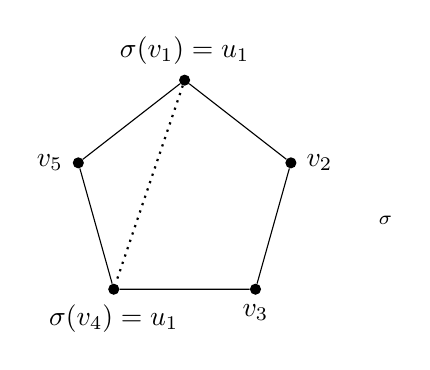
\begin{tikzpicture}[scale=1.5]
        \node[circle, fill, scale=0.015cm, label=above:{$\sigma(v_1)= u_1$}] (l1) at (0, 1) { };
        \node[circle, fill, scale=0.015cm, label=right:{$v_2$}] (l2) at (0.9, 0.30) { };
        \node[circle, fill, scale=0.015cm, label=below:{$v_3$}] (l3) at (0.6, -0.77) {};
        \node[circle, fill, scale=0.015cm, label=below:{$\sigma(v_4)=u_1$}] (l4) at (-0.6, -0.77) {};
        \node[circle, fill, scale=0.015cm, label=left:{$v_5$}] (l5) at (-0.9, 0.30) {};
        \draw (l1) -- (l2) -- (l3) -- (l4) -- (l5) -- (l1);
        \draw[dotted, thick] (l1) -- (l4);
        \node at (1.7, -0.2) { $\stackrel{\sigma}{\implies}$ };
    \end{tikzpicture}
    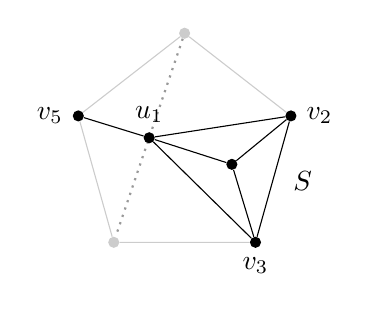
\begin{tikzpicture}[scale=1.5]
        \node[circle, fill, opacity=0.2, scale=0.015cm] (l1) at (0, 1) {};
        \node[circle, fill, opacity=0.2, scale=0.015cm] (l4) at (-0.6, -0.77) {};
        \node[circle, fill, scale=0.015cm, label=above:{$u_1$}] (y1) at (-0.3, 0.115) {};

        \node[circle, fill, scale=0.015cm, label=right:{$v_2$}] (l2) at (0.9, 0.30) { };
        \node[circle, fill, scale=0.015cm, label=below:{$v_3$}] (l3) at (0.6, -0.77) {};
        \node[circle, fill, scale=0.015cm, label=left:{$v_5$}] (l5) at (-0.9, 0.30) {};
        \node[circle, fill, scale=0.015cm] (s) at (0.4, -0.11) { };
        \node (s1) at (1.0, -0.25) { $S$ };

        \draw (s) -- (y1);
        \draw (s) -- (l3);
        \draw (s) -- (l2);
        \draw (l5) -- (y1) -- (l2) -- (l3) -- (y1);
        \draw[dotted, thick, opacity=0.4] (l1) -- (l4);
        \draw[opacity=0.2] (l5) -- (l1) -- (l2);
        \draw[opacity=0.2] (l3) -- (l4) -- (l5);
    \end{tikzpicture}
    \caption{First, the two vertices $v_1$ and $v_4$ are contracted to the same vertex $y_1$, then we turn the contracted graph into $S$.  }
    \label{fig:contract}
\end{figure}

A contraction maps the vertices of $R$ to the vertices of $\sigma(R)$. Those vertices that are mapped to the same vertex are contracted. This mapping allows us to directly convert a ring coloring $x(u)$ of $S$ to a ring coloring $x(\sigma(v))$ of $R$. Note that the reducers we used for $k$-reducibility used the identity contraction $\sigma(v) = v$, which does not contract any edges.

\begin{definition}
    A ring contraction $\sigma(v)$ on $R$ is a map from the vertices of $R \mapsto \sigma(R)$. Neighboring vertices of $R$ may not be mapped to the same vertex.
\end{definition}

\begin{definition}
    $\sigma_{id}(v) = v$ is the \emph{identity contraction}.
\end{definition}

\begin{definition}
    A reducer $(S,\sigma)$ of a configuration $\confg$ consists of a contraction $\sigma(v)$ on $R$ and a graph $S < \confg$ whose boundary is the contracted ring $\sigma(R)$.
\end{definition}

\begin{definition}
    The set of reducer-constrained ring colorings $\Phi(S, \sigma)$ consists of all the colorings $x(\sigma(v))$ with $x(u)$ a boundary coloring of $S$.
\end{definition}


The reducer for $\ber$ is given in Figure \ref{fig:bernhart_reducer}. It consists of two contractions and a single extra edge added by $S$ in the middle. The mapping of colorings from $S$ to $R_8$ are given below. It is helpful to think of a reducer solely as a set of constraints.

\begin{equation}
    v_1\;\textbf{u}_\textbf{2}\;v_3\;v_5\;\textbf{u}_\textbf{1}\;v_7 \quad\mapsto \quad v_1\;\textbf{u}_\textbf{2}\;v_3\;\textbf{u}_\textbf{2}\;v_5\;\textbf{u}_\textbf{1}\;v_7\;\textbf{u}_\textbf{1}.
\end{equation}

\begin{figure}[!ht]
    \centering
    \begin{tikzpicture}[scale=1.5, mid arrow/.style={
        postaction={ decorate, decoration={ markings, mark=at position 0.6 with { \arrow[black]{>>} } } } }]
        \node[circle, fill, scale=0.015cm, label=left:$v_1$] (l1) at (-2, 0) { };
        \node[opacity=0.4] at (-1.2, 1.1) { $v_8$ };
        \node[circle, fill, scale=0.015cm, opacity=0.2] (l2) at (-1, 1) { };
        \node[opacity=0.4] at (-1.2, -1.1) { $v_2$ };
        \node[circle, fill, scale=0.015cm, opacity=0.2] (l4) at (-1, -1) {};

        \node[circle, fill, scale=0.015cm, label=right:$v_5$] (r1) at (2, 0) {};
        \node[opacity=0.4] at (1.2, 1.1) { $v_6$ };
        \node[circle, fill, scale=0.015cm, opacity=0.2] (r2) at (1, 1) {};
        \node[opacity=0.4] at (1.2, -1.1) { $v_4$ };
        \node[circle, fill, scale=0.015cm, opacity=0.2] (r4) at (1, -1) {};

        \node[circle, fill, scale=0.015cm, label=above:$v_7$] (b1) at (0, 1) {};
        \node[circle, fill, scale=0.015cm, label=below:$v_3$] (b2) at (0, -1) {};
        \node[circle, fill, scale=0.015cm, label=below left:$u_1$] (u1) at (0, 0.5) {};
        \node[circle, fill, scale=0.015cm, label=above left:$u_2$] (u2) at (0, -0.5) {};

        \draw[opacity=0.2] (l1) -- (l2) -- (b1) -- (r2) -- (r1) -- (r4) -- (b2) -- (l4);
        \draw [mid arrow, opacity=0.3] (l1) -- (l4);
        \draw (l1) -- (u1) -- (r1) -- (u2) -- (l1);
        \draw (b1) -- (u1);
        \draw (b2) -- (u2);
        \draw (u1) -- (u2);
        \draw[dotted, thick, opacity=0.4] (l2) -- (u1) -- (r2);
        \draw[dotted, thick, opacity=0.4] (l4) -- (u2) -- (r4);

    \end{tikzpicture}
    \caption{The reducer $S$ of the Bernhart Diamond $\bir$. It forces that $v_2 =v_4 \neq v_6 = v_8$. The contractions force the same colors on pairs of vertices, while the added edges force different colors. }
    \label{fig:bernhart_reducer}
\end{figure}

In the next section we will show that the red generated colorings in Figure \ref{table:bernhart} are actually in $\maxi{\ber}$, therefore $\Phi(S,\sigma) \subset \maxi{\ber}$. As a result, we may replace $\ber$ by its reducer $S$ and be guaranteed that any coloring for $S$ can be reconfigured ot a valid coloring. This is the essence of C-reducibility.
\begin{definition}
    A configuration $\confg$ is C-reducible if $\Phi(S,\sigma) \subset \overline{\Phi}(\confg)$ for some reducer $(S,\sigma)$.
\end{definition}

\begin{figure}[!ht]
    \centering
    \begin{tikzpicture}[scale=1.0]
        \draw (0, 0) ellipse (3cm and 1.8cm);
        \draw (0, -0.3) ellipse (2cm and 1.2cm);
        \draw[fill opacity=0.4, pattern=north east lines] (0.8, -0.6) ellipse (0.8cm and 0.6cm);
        \draw[dotted, thick] (-0.7, -0.4) ellipse (1.0cm and 0.6cm);

        \node at (0.9, -0.6) { $\Phi_0(\confg)$ };
        \node at (0.3, 0.35) { $\overline{\Phi}(\confg)$ };
        \node at (0, 1.35) { $\Phi(n)$ };
        \node at (-0.8, -0.4) { $\Phi(S, \sigma)$ };
    \end{tikzpicture}

    \caption{The max-implying set includes all generated colorings of $\Phi(S,\sigma)$.  }
    \label{fig:cred}
\end{figure}

For any given configuration, there are only a finite number of reducers $(S,\sigma)$ possible. Therefore, it is feasible to simply test all possible reducers for the condition $\Phi(S,\sigma) \subset \maxi{\confg}$. 